\section{Compiler Implementation}\label{sec:compiler}



%-----------------------------------------------------------------------------
\subsection{Omni XMP Compiler Framework}
%-----------------------------------------------------------------------------

\begin{figure}[tbh]
 \begin{center}
  % trimはleft bottom right topの順
  %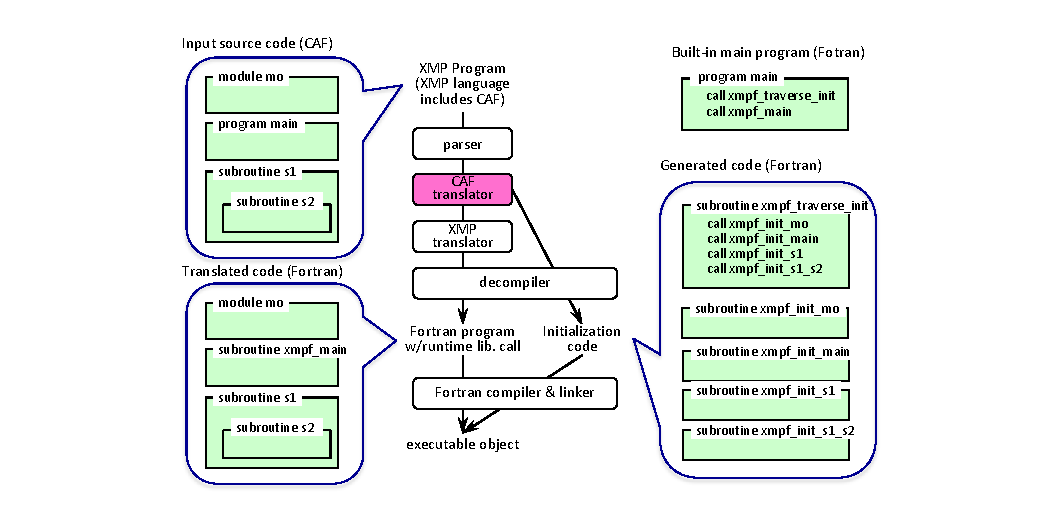
\includegraphics[scale=0.55,trim=6cm 0cm 4cm 6cm,clip]{figs/translator-tmp.pdf}
  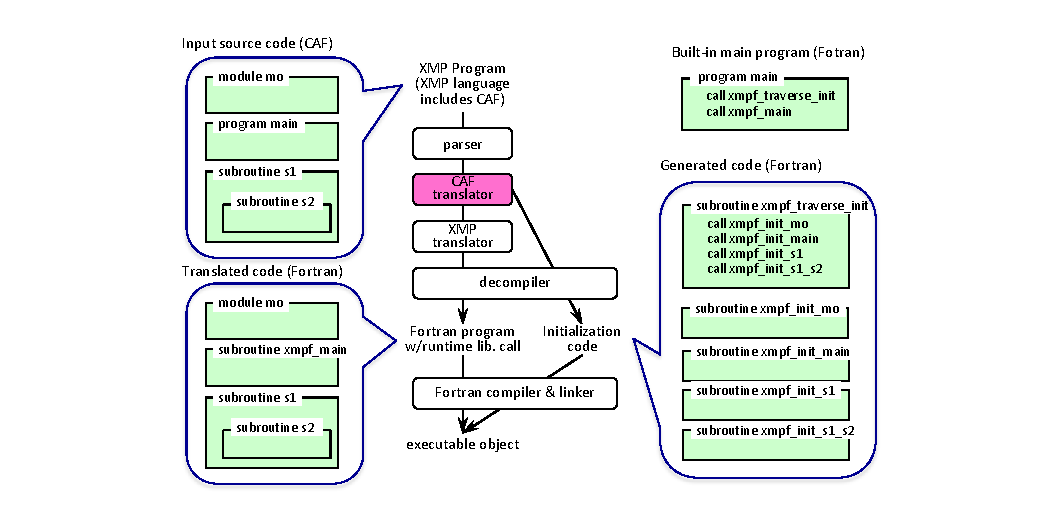
\includegraphics[trim=30mm 0mm 20mm 7mm, scale=1.0]{figs/translator-tmp.pdf}
  \caption{XMP compiler and an example of coarray program compilation}
  \label{fig:translator}
  %-- 修正すべき箇所
  CAF translator $\rightarrow$ coarray translator
 \end{center}
\end{figure}

The CAF translator was added into the Omni XMP compiler as shown in Figure~\ref{fig:translator}.
The Omni XMP compiler is a source-to-source translator that converts XMP programs into 
the base language (Fortran or C).  The component `coarray translator' is located in 
front of the XMP translator to solve coarray features previously. The output of the decompiler 
is a standard Fortran/C program that may include calls to the XMP runtime library.

In order to allocate and register static coarray variables prior to the execution of the user program, 
the built-in main program is made in order to call the initialization routine 
{\tt xmpf\_traverse\_init} followed by user’s main program.
{\tt xmpf\_traverse\_init} is generated by the coarray translator to call initialization 
routines (e.x., {\tt xmpf\_init\_foo}) corresponding to user-defined procedures (e.x., {\tt foo}).



%-----------------------------------------------------------------------------
\subsection{PUT/GET Communication}
%-----------------------------------------------------------------------------

To avoid disturbing the execution on the remote image, PUT and GET communications
are implemented always using Remote Direct Memory Access (RDMA) provided by 
the communication library (except coarrays with pointer/allocatable structure components). 
In contrast, local data access is selective between using Direct Memory Access (DMA) or
using a local buffer. And the suitable algorithm differs depending on the 
relationship of the three parameters, the size of the local buffer $B$ and the 
local and remote contiguous lengths $N_L$ and $N_R$.
The Fortran syntax guarantees that $N_L$ is a multiple of $N_R$ or $N_R$ is a multiple of $N_L$.

Table~\ref{tab:putget} summarizes our algorithm for PUT/GET communication for five cases.
The unit size is the chunk length of the PUT/GET communication.
Case~0 shows the algorithm using RDMA-DMA PUT/GET communication and Cases~1 through~4
shows the algorithms using RDMA and local-buffering. 
Due to its strict condition, the DMA scheme is rarely used.
And it is not always faster than the buffering scheme cases~2 and~3 because of the 
difference of the unit sizes. The merit of cases~2 and~3 is that the unit size 
is extended to a multiple of $N_L$ by gathering number of short contiguous data in the buffer,
or by scattering from the buffer into number of short contiguous data.

\begin{table}[tbh]
 \caption{Summary of the PUT/GET algorithm related to $N_L$, $N_R$ and $B$}
 \label{tab:putget}
 \begin{flushleft}
  \begin{tabular}{|c||c|c|c|}
\hline
case & scheme 
& condition 
& unit size
\\
\hline
\hline
0 & DMA   
& Local data is registered.
& $\min(N_L, N_R)$   
\\
\hline
1 & buffering 
& $N_R \leq B,~ N_R \leq N_L$
& $N_R$
\\
\cline{1-1} \cline{3-4}
2 &
& $N_L < N_R \leq B$
& $N_R$
\\
\cline{1-1} \cline{3-4}
3 &
& $N_L < B < N_R$
& multiple of $N_L$ and up to $B$
\\
\cline{1-1} \cline{3-4}
4 &
& $B < N_R,~ B \leq N_L$
& $B$ (or less than $B$ at last)
\\
\hline
  \end{tabular}
 \end{flushleft}
 \begin{flushleft}
  \begin{tabular}{|c||l|l|}
\hline
case 
& PUT action for every unit
& GET action for every unit
\\
\hline
\hline
0 
& put once
& get once
\\
\hline
1 
& buffer once and put once
& get once and unbuffer once
\\
\hline
2 
& buffer for each $N_L$, and put once
& get once, and unbuffer for each $N_L$
\\
\hline
3 
& buffer for each $N_L$, and put once
& get once, and unbuffer for each $N_L$
\\
\hline
4 
& buffer once and put once
& get once and unbuffer once
\\
\hline
  \end{tabular}
 \end{flushleft}
\end{table}




\subsubsection{static coarrayの高速化}

全部まとめて先にallocするコンパイラ技術

定数評価、構造体の大きめな見積り

\subsubsection{allocatable coarrayの高速化}

lower level communication libraryに合わせてallocation methodを選択

runtimelibshare事前に巨大領域を取る

実行時allocのコストが大きいとき


runtimeliballocation実行時allocのコストが小さいとき

\subsubsection{contiguity検出による高速化}
次元を跨ぐ連続性抽出

\subsubsection{バッファリング}
有限サイズ、基礎データから、nlocal, nremote, nbufの関係でアルゴリズム
commpilerallocationfortranがallocateしてregisterできるとき



